\chapter{Workflow} % Main chapter title

\label{Chapter 4} 
\lhead{Chapter 4. \emph{Workflow}} 

In this chapter, we will discuss the workflow of our project and some algorithm.



\section{Workflow}
In this section, we will discuss the proposed workflow.
It takes RGB frame and outputs labelled feature as Keyfeature\textbf{(KF)} and motion frame \textbf{(MF)}. Classification of Keyfeature\textbf{(KF)} or non-motion frame and motion frame \textbf{(MF)} comprises the following parts:

\subsection{Background Subtraction Module}

\subsubsection{RGB image to Grayscale image:} 
It takes a colour image(RGB channels) of size 480 x 640. After that, the RGB image is converted to grayscale (single grayscale channel) of size 480 x 640. It helps in decreasing the complexity of the introduced method. Grayscale pixel’s value is computed by the weighted sum of the corresponding red, green, and blue pixels as:

\[\Large GrayFrame(i, j) = 0.299 \ast Frame(i, j)_R\]
\[\Large + 0.587 \ast Frame(i, j)_G\]
\[\Large + 0.144 \ast Frame(i, j)_B\]
\[\Large Where 1 \leqslant i \leqslant 480 and 1 \leqslant j \leqslant 640\]

\subsubsection{Background Removal}

\begin{figure}[H]
    \centering
    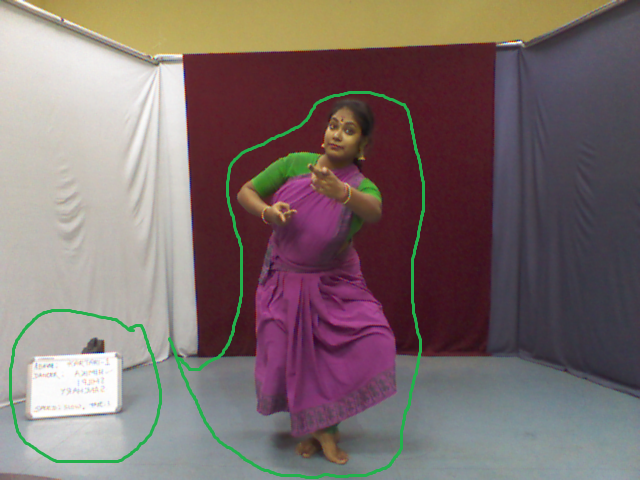
\includegraphics[scale= 0.7]{./Pictures/background_image.png}
    \caption{Redundant information highlighted}
    \label{fig:Ch04F001}
\end{figure}
Dancer image contains lots of redundant information which is not required for us—for example, background image or board on the side of the dancer, as shown in Figure \ref{fig:Ch04F001}. 

\begin{figure}[H]
\centering
  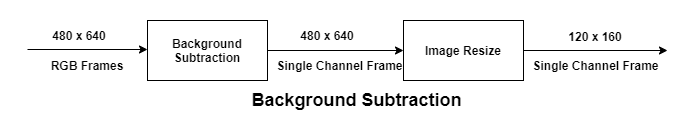
\includegraphics[scale= 0.6]{./Pictures/Algorithm-Background_Subtration.png}
  \caption{Background Subtraction}
  \label{fig:Ch04F002}
\end{figure}


Kinect depth data has 16-bit information, which consists of 3 bits which signify player index and the remaining 13 bits mean depth data. The depth data is the distance between the dancer and the camera lens. It uses the following algorithm as shown in Figure \ref{fig:Ch04F003}

\begin{figure}[H]
\centering
  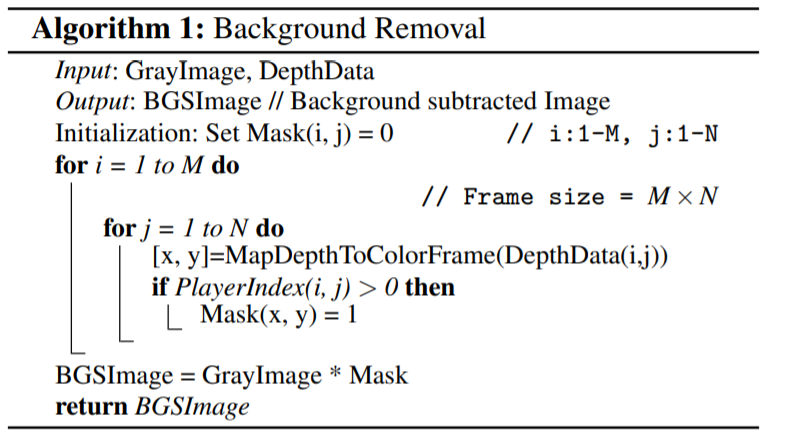
\includegraphics[scale= 0.7]{./Pictures/algo_image.png}
  \caption{Background Subtraction algorithm}
  \label{fig:Ch04F003}
\end{figure}

Since we are calculating optical flow which using motion information, so, we would remove the background from a grey image and retain only the information dancer portion. We would use depth stream information from Kinect depth
data as shown on Figure \ref{fig:Ch04F002} and \ref{fig:Ch04F003}.

\subsubsection{Resize Image}
After that, the image is resized to size $120 \ast 160$. We have used OpenCV, \texttt{\textbf{cv2.resize()}} function for this purpose. This function takes an image of size $480 \ast 640$ and resizes the image source down to size $120 \ast 160$, as shown in Figure \ref{fig:Ch04F002}
    





\subsection{Preprocessing Example (Backgroud Subtraction)}
\begin{figure}
    \centering
    \subfigure[]{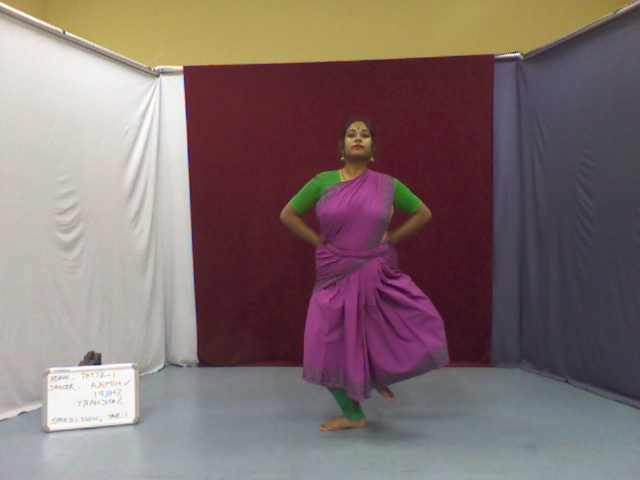
\includegraphics[width=0.22\textwidth]{Pictures/1_1.png}} 
    \subfigure[]{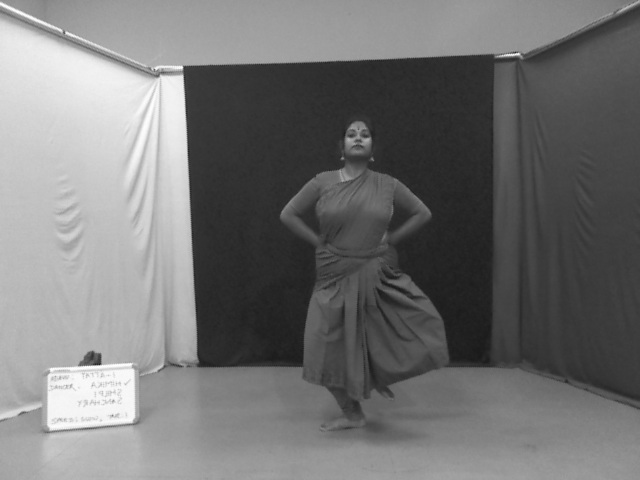
\includegraphics[width=0.22\textwidth]{Pictures/1_2.png}} 
    \subfigure[]{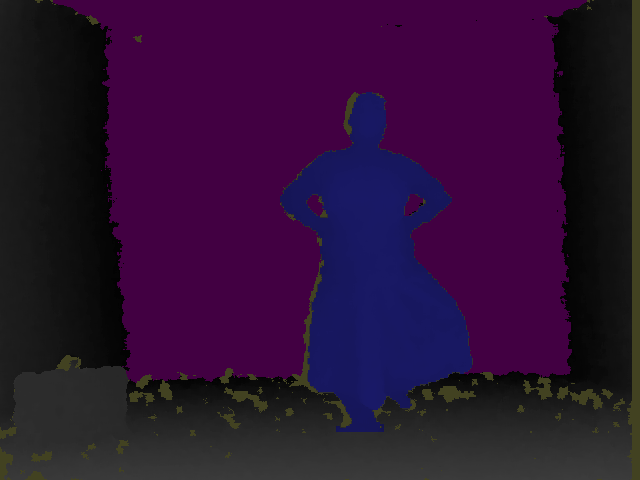
\includegraphics[width=0.22\textwidth]{Pictures/1_3.png}}
    \subfigure[]{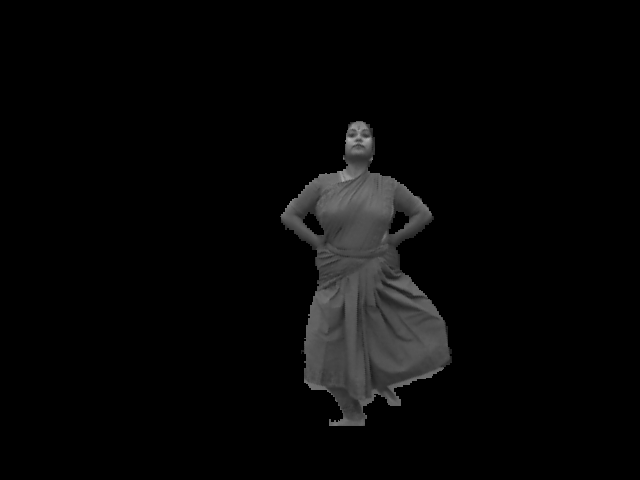
\includegraphics[width=0.22\textwidth]{Pictures/1_4.png}}
    \caption{(a) RGB (b) Grey (c) Depth Frame (d) Single channel}
    \caption{Tatta-$>$Variation-$>$Dancer 1}
    \label{fig:Ch04F004}
\end{figure}
 
\begin{figure}
    \centering
    \subfigure[]{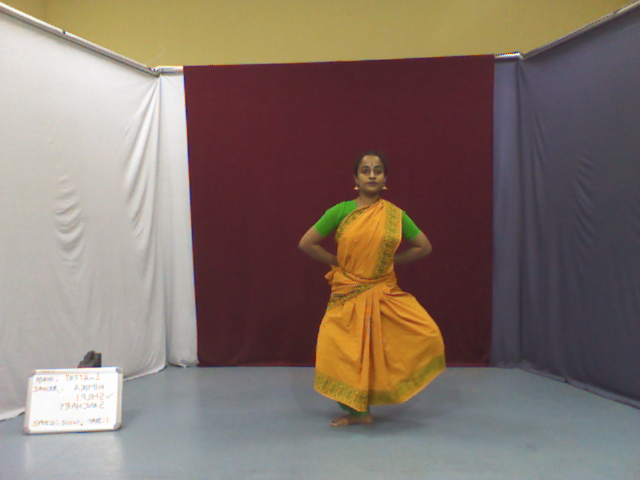
\includegraphics[width=0.22\textwidth]{Pictures/2_1.png}} 
    \subfigure[]{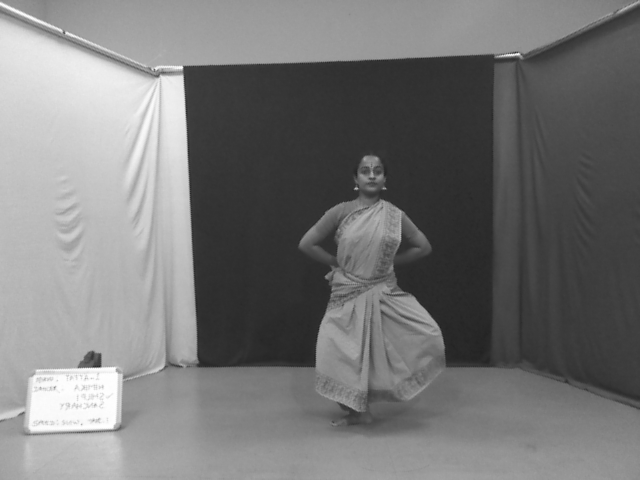
\includegraphics[width=0.22\textwidth]{Pictures/2_2.png}} 
    \subfigure[]{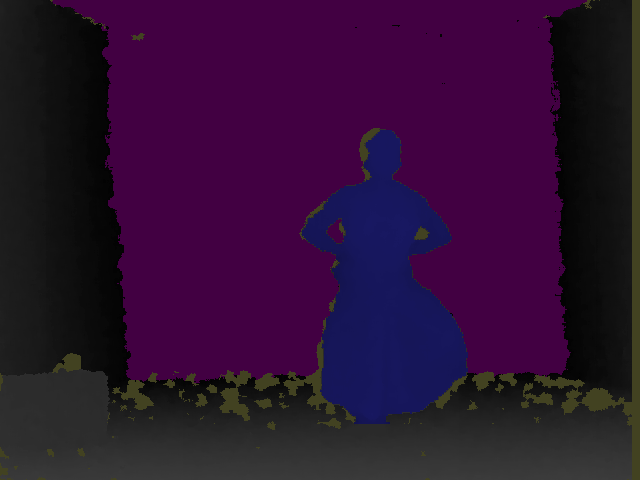
\includegraphics[width=0.22\textwidth]{Pictures/2_3.png}}
    \subfigure[]{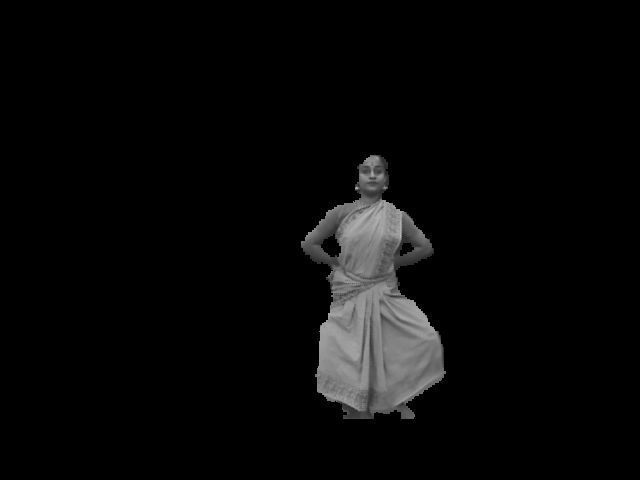
\includegraphics[width=0.22\textwidth]{Pictures/2_4.png}}
    \caption{(a) RGB (b) Grey (c) Depth Frame (d) Single channel}
    \caption{Tatta-$>$Variation-$>$Dancer 2}
    \label{fig:Ch04F005}
\end{figure}
 
 \begin{figure}
    \centering
    \subfigure[]{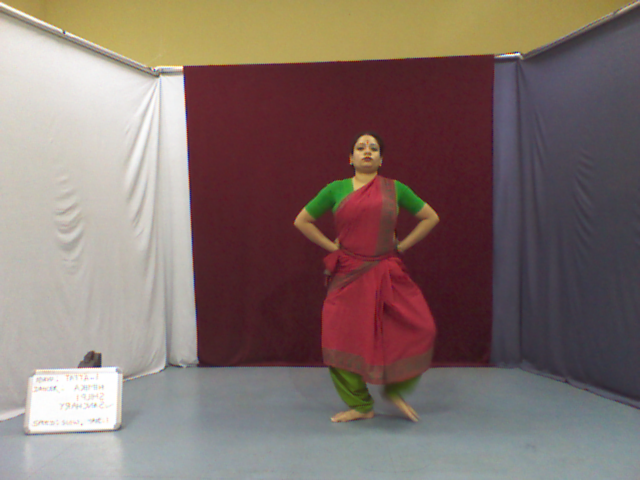
\includegraphics[width=0.22\textwidth]{Pictures/3_1.png}} 
    \subfigure[]{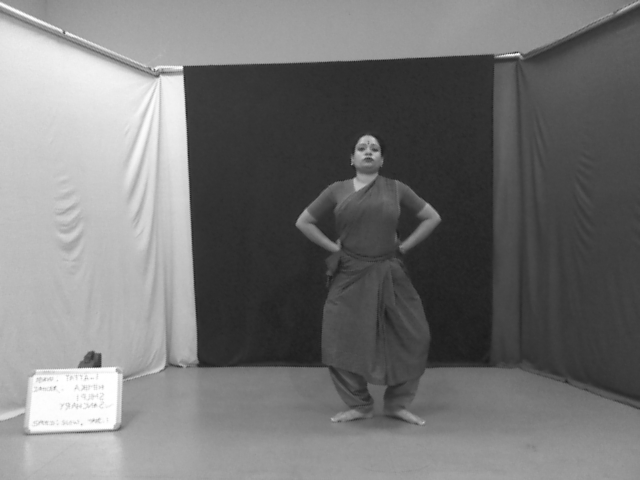
\includegraphics[width=0.22\textwidth]{Pictures/3_2.png}} 
    \subfigure[]{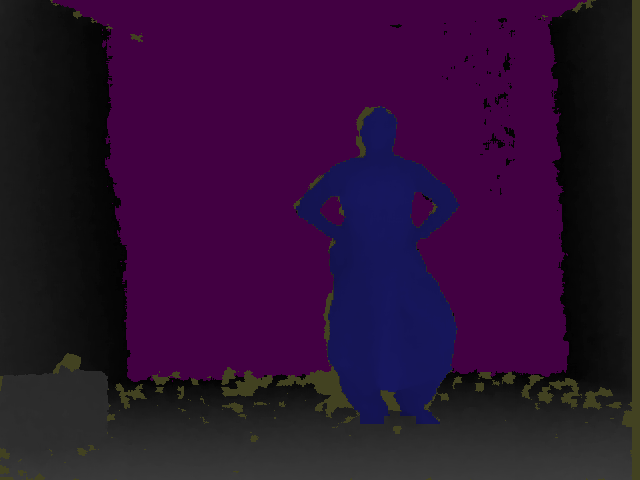
\includegraphics[width=0.22\textwidth]{Pictures/3_3.png}}
    \subfigure[]{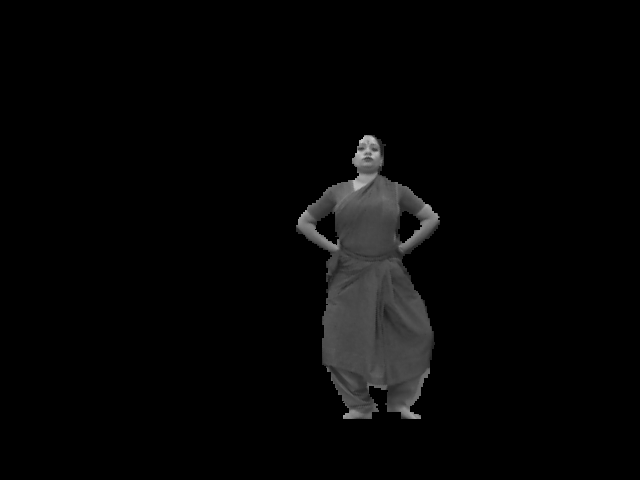
\includegraphics[width=0.22\textwidth]{Pictures/3_4.png}}
    \caption{(a) RGB (b) Grey (c) Depth Frame (d) Single channel}
    \caption{Tatta-$>$Variation-$>$Dancer 3}
    \label{fig:Ch04F006}
\end{figure}

It is the example of background removal as shown in Figure \ref{fig:Ch04F004}, \ref{fig:Ch04F005} and \ref{fig:Ch04F006}.
 
 
    
    
    
    
\subsection{Feature Extraction Module}

\begin{figure}[H]
  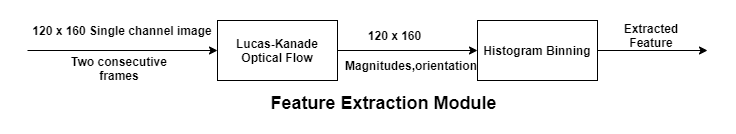
\includegraphics[scale= 0.5]{./Pictures/Algorithm-Feature_Extraction.png}
  \caption{Feature Extraction}
  \label{fig:Ch04F007}
\end{figure}
In this section, we will explain the feature extraction method used. This feature would be used for classification KeyFrame and motion frame (non-KeyFrame) in given Bharatnatyam adavu video. Lucas-Kanade optical flow is calculated. Two consecutive frames of size 120 x 160 single-channel images are taken as input. Lucas-Kanade optical flow method yield a matrix of size 120*160, which contains magnitudes and orientations. These are considered as input for Histogram binning. Histogram binning methods depend on the approaches we have taken. These would output the final feature vector for labelling. Different type of Histogram binning is used to feature descriptor.



    
\subsubsection{Estimate Optical Flow: Lucas-Kanade Method}


'opticalFlowLK' is used to estimate the optical flow using the Lucas-Kanade method \citep{barron1994performance}. This function generates an optical flow object for determining the direction(displacement) and speed of an apparent moving object using the Lucas-Kanade method(optical flow calculation method).

\begin{figure}
    \centering
    \subfigure[]{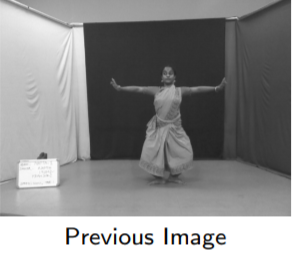
\includegraphics[width=0.32\textwidth]{Pictures/image1.png}} 
    \subfigure[]{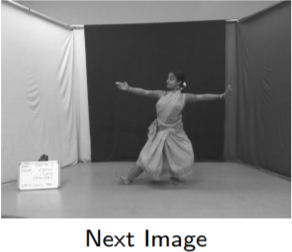
\includegraphics[width=0.32\textwidth]{Pictures/image2.png}} 
    \subfigure[]{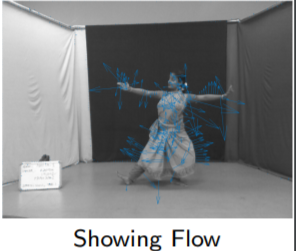
\includegraphics[width=0.32\textwidth]{Pictures/image3.png}} 
    \caption{(a) Previous Image (b) Next Image (c) Showing Image}
    \label{fig:Ch04007}
\end{figure}

\subsubsection{Algorithms}
\begin{enumerate}
    \item Input: Two consecutive images
    \item Output: Optical flow / velocity vector $(V_x, V_y) = (u, v)$ for each pixel
    \item Assumption: Brightness/ Intensity doesn’t change with time. So, $I(x, y, t) = I(x + u, y + v, t)$
\end{enumerate}

\begin{itemize}
    \item $I_x, I_y$, and It are the spatiotemporal image brightness derivatives.
    \item $u$ is the horizontal velocity vector.
    \item $v$ is the vertical velocity vector.
\end{itemize}
\[\huge I_xu+I_yv+I_t=0\]

\subsubsection{Lucas-Kanade Method}
The Optical flow constraint equation is solved using the Lucas-Kanade for $u$ \& $v$, the method splits the initial image into smaller segments and assumes a consistent velocity in each region.
A weighted and least-square fit is performed on the optical flow constraint equation to a consistent model for $[u  v]^T$ in each section of $\Omega$.
The given process achieves that fit by minimizing following the given equation:
\[\sum_{x \in Q} W^2 [I_xu + I_yv + I_t]^2\]

W is a window function for the center of each section. The solution to the minimization problem is:

\[\begin{bmatrix} & \sum W^2I_x^2 & \sum W^2I_xI_y \\
& \sum W^2I_yI_x & \sum W^2I_y^2 \end {bmatrix}\begin{bmatrix} & u\\ & v\end{bmatrix} = -\begin{bmatrix} & \sum W^2I_xI_t \\
& \sum W^2I_yI_t \end{bmatrix}\]


\subsubsection{Histogram Binning}
Histograms are utilized broadly as non-parametric frequency estimators for visualizing data and for obtaining extract quantities. However, the values of frequency estimators depend on the number of bins taken for the Histogram. There are some rules to determine bins number. For example, Generally, 5-20 bins numbers are satisfactory. As in the case of Matlab, ten(10) bins number is used as a default parameter.
We have used following Histogram binning method:

\begin{enumerate}
    \item Global Histogram using only magnitudes of optical flow.
    \item Global Histogram using magnitudes and orientation of optical flow.
    \item Fractional Histogram Binning using magnitudes and orientation of     optical flow taken over $8 \ast 8$ cell.
\end{enumerate}
    

\subsection{Training Module}
\begin{figure}[H]
    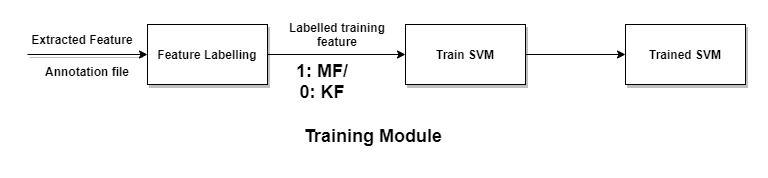
\includegraphics[scale= 0.6]{./Pictures/Algorithm-Training_Module.png}
    \caption{Training Module}
    \label{fig:Ch04F012}
\end{figure}
Extracted feature from the previous module with the help of annotation file is used to train the SVM classifier as shown in Figure \ref{fig:Ch04F012}.


\subsubsection{Feature Labeling}
Extracted feature and annotation file in ’CSV’ format is taken as input for feature labelling. The feature is marked as 1 for motion frame as this is our primary and as 0 for the KeyFrame as shown in Figure \ref{fig:Ch04F012}.



\subsubsection{Training SVM}
SVM(Support vector machine) is a mechanism of pattern identification that has a precise theoretical basis. So, we used a linear SVM classifier for feature labelling whether it is KeyFrame or motion frame.
Data set means a set of all motion frames and KeyFrame (non-motion frame).
The features are generated by Histogram binning in the previous section.
The dataset containing all frames was randomly separated into two datasets, i.e., training dataset and test dataset. The training dataset includes 80 per cent, both motion frames, and KeyFrames. Test dataset contains 20 per cent also contain both motion frames and KeyFrames.



\begin{lstlisting}
kernel = 'linear'
#Create a svm Classifier
clf = svm.SVC(kernel=kernel)  # Linear Kernel

#Train the model using the training sets
clf.fit(X_train, y_train)
\end{lstlisting}


    
    
 \subsection{Testing Module}
We would use the test dataset, i.e., the test feature vector is used on trained SVM. This trained SVM would label a given frame, whether it is motion frame(MF:1) or KeyFrame (KF:0) as shown in Figure \ref{fig:Ch04F013}.

 \begin{figure}[H]
  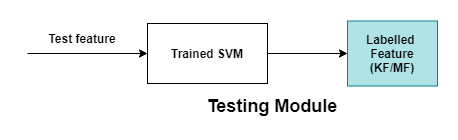
\includegraphics[scale= 0.7]{./Pictures/Algorithm-Testing_Module.png}
  \caption{Testing Module}
  \label{fig:Ch04F013}
\end{figure}
 
 \subsubsection{Evaluation metrics}
Some motion frames will be detected as KeyFrame and some KeyFrame will be detected as motion frame.

We have used four usually accepted criteria, i.e.,
\begin{enumerate}
    \item Accuracy
    \item Precision
    \item Recall
    \item F1-Score
\end{enumerate}
It is used for the evaluation of prediction performance of constructed SVM binary classifier models. The accuracy is the number of correctly predicted KeyFrame and motion frame out of the total number of given frames. The precision is the number of actual KeyFrame and motion frame out of predicted KeyFrame and motion frame.
The recall is the number of correctly predicted KeyFrame and motion frame out of actual KeyFrame and motion frame
The F1 score value is a merged value of recall and precision.



\textbf{\[F1Score = 2* \frac{Precision * Recall}{Precisin + Recall} \]}

KeyFrame accuracy is determined by following formula:
\[Accuracy_{KF} = \frac{KF_{Detected}}{KF_{Total}}\]
where $Accuracy_{KF}$ : Accuracy of KeyFrame,\newline 
$KF_{Detected}$ : Number of detected KeyFrame \& \newline
$KF_{Total}$ : Total Number of KeyFrame.\newline

\[Accuracy_{MF} = \frac{MF_{Detected}}{MF_{Total}}\]
where $Accuracy_{MF}$ : Accuracy of Motion Frame,\newline 
$MF_{Detected}$ : Number of detected Motion Frame \& \newline
$MF_{Total}$ : Total Number of Motion Frame.\newline

No doubt we have computed for both motion frame(MF) and KeyFrame(KF). Our objective is to detect motion key(MF).

True Positive(TP) = Motion Frame
True Negative(TN) = Key Frame

\textbf{TP} = Motion frame when it was Motion frame.\newline
\textbf{TN} = Key frame when it was Key frame.\newline
\textbf{FP} = Motion frame when it was Key frame.\newline
\textbf{TN} = Key frame when it was Motion frame.\newline

\[
Accuracy_{Total} = \frac{KF_{Correct\_Detected} + MF_{Correct\_Detected}}{KF_{Total} + MF_{Total}}
\]
